% This is text associated with the open textbook "Open Electromagnetics"
% See immediately below for author, date
% This work is licensed under the Creative Commons Attribution-ShareAlike 4.0 International License. (CC BY-SA 4.0) 
% To view a copy of the license, visit http://creativecommons.org/licenses/by-sa/4.0/

%ORB TITLE Optical Fiber: Method of Operation
%ORB AUTHOR 0        # S.W. Ellingson, Virginia Tech (ellingson@vt.edu)
%ORB DATE 20191123   # yyyymmdd
%ORB ABSTRACT 

\label{m0178_Optical_Fiber_Method_of_Operation} % <-- Must match name of this file and module directory name.  Don't mess with this!
\index{optical fiber|(}

In its simplest form, optical fiber consists of concentric regions of dielectric material as shown in Figure~\ref{m0178_fOF}.
%
\begin{figure}[b!] % <--- "[b]" for first figure in section *only*; delete for 2nd and subsequent figures
\begin{center}
\pdftooltip{{  % note double braces
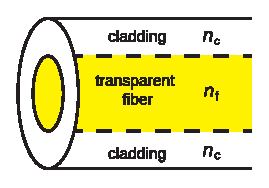
\includegraphics[width=2in]{modules/m0178_fOF.eps} 
% https://commons.wikimedia.org/wiki/File:Figure_8.1-01.svg
}}{Two concentric cylinders. The space between inner and outer cylinders is labeled cladding, small n subscript c, and the inner cylinder is labeled transparent fiber, small n subscript f.}
\end{center}
\centerline{\scriptsize 
\copyright~\hyperref[m0178_fOF_Credit]{S.\ Lally} 
\href{https://creativecommons.org/licenses/by-sa/4.0/}{CC BY-SA 4.0} 
} % \centerline 
\caption{
\label{m0178_fOF}
Construction of the simplest form of optical fiber.
}
\end{figure} 
%
A cross-section through the fiber reveals a circular region of transparent dielectric material through which light propagates.
This is surrounded by a jacket of dielectric material commonly referred to as \emph{cladding}.
\index{cladding}

A characteristic of the design of any optical fiber is that the permittivity of the fiber is greater than the permittivity of the cladding.
As explained in Section~\ref{m0169_Total_Internal_Reflection}, this creates conditions necessary for total internal reflection.
\index{total internal reflection}
The mechanism of total internal reflection contains the light within the fiber.   

In the discipline of optics, the permittivity of a material is commonly quantified in terms of its \emph{index of refraction}.
\index{index of refraction}
Index of refraction is the square root of relative permittivity, and is usually assigned the symbol $n$.
Thus, if we define the relative permittivities 
$\epsilon_{r,f} \triangleq \epsilon_f / \epsilon_0$ for the fiber and
$\epsilon_{r,c} \triangleq \epsilon_c / \epsilon_0$ for the cladding, 
then
%
\begin{flalign}
n_f &\triangleq \sqrt{\epsilon_{r,f}} \\
n_c &\triangleq \sqrt{\epsilon_{r,c}}
\end{flalign}
and
%
\begin{equation}
n_f > n_c 
\end{equation}
  
Figure~\ref{m0178_fTIR} illustrates total internal reflection in an optical fiber.
In this case, a ray of light in the fiber is incident on the boundary with the cladding.
We may treat the light ray as a uniform plane wave.  
To see why, consider that optical wavelengths range from 120~nm to 700~nm in free space.
Wavelength is slightly shorter than this in fiber; specifically, by a factor equal to the square root of the relative permittivity.
The fiber is on the order of millimeters in diameter, which is about 4 orders of magnitude greater than the wavelength.
Thus, from the perspective of the light ray, the fiber appears to be an unbounded half-space sharing a planar boundary with the cladding, which also appears to be an unbounded half-space.  
%
\begin{figure} % <--- "[b]" for first figure in section *only*; delete for 2nd and subsequent figures
\begin{center}
\pdftooltip{{  % note double braces
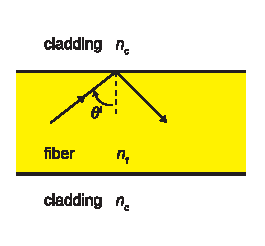
\includegraphics[width=2in]{modules/m0178_fTIR.eps} 
% https://commons.wikimedia.org/wiki/File:Internal_Reflection_in_Optical_Fiber.svg
}}{A cross-sectional view of a fiber shows a ray approaching the edge of the inner fiber at an angle theta superscript i measured from the vertical. The ray is reflected back into the fiber. Cladding, small n subscript c, fills the area outside the fiber.}
\end{center}
\centerline{\scriptsize 
\copyright~\hyperref[m0178_fTIR_Credit]{S.\ Lally} 
\href{https://creativecommons.org/licenses/by-sa/4.0/}{CC BY-SA 4.0} 
} % \centerline 
\caption{
\label{m0178_fTIR}
Total internal reflection in optical fiber.
}
\end{figure} 

Continuing under this presumption, the criterion for total internal reflection is (from Section~\ref{m0169_Total_Internal_Reflection}):
%
\begin{equation}
\theta^i \ge \arcsin\sqrt{\frac{\epsilon_{r,c}}{\epsilon_{r,f}}} = \arcsin\frac{n_c}{n_f}
\label{m0178_eCAnm}
\end{equation}
%
As long as rays of light approach from angles that satisfy this criterion, the associated power remains in the fiber, and is reflected onward.
Otherwise, power is lost into the cladding.

%%%%%%%%%%%%%%%%%%%%%%%%%%%%%%%%%%%%%%%%%%%%%%%
%ORB EXAMPLE
~\\ \begin{example} 
\begin{mdframed}[backgroundcolor=brown!20,linecolor=brown!20]\raggedright
Critical angle for optical fiber.
\\~\\
Typical values of $n_f$ and $n_c$ for an optical fiber are 1.52 and 1.49, respectively.  What internal angle of incidence is required to maintain total internal reflection?

{\bf Solution}. Using Equation~\ref{m0178_eCAnm}, $\theta^i$ must be greater than about $78.8^{\circ}$.  
In practice this is quite reasonable since we desire light to be traveling approximately parallel the axis of the fiber ($\theta^i\approx 90^{\circ}$) anyway.
\end{mdframed}
% note figures will need to go between "\end{mdframed}" and "\end{example}"
\end{example}
%%%%%%%%%%%%%%%%%%%%%%%%%%%%%%%%%%%%%%%%%%%%%%%

The total internal reflection criterion imposes a limit on the radius of curvature of fiber optic cable.
If fiber optic cable is bent such that the radius of curvature is too small, the critical angle will be exceeded at the bend.
This will occur even for light rays which are traveling perfectly parallel to the axis of the fiber before they arrive at the bend.

Note that the cladding serves at least two roles.  
First, it determines the critical angle for total internal reflection, and subsequently determines the minimum radius of curvature for lossless operation of the fiber.
Second, it provides a place for the evanescent surface waves associated with total internal reflection (Section~\ref{m0170_Evanescent_Waves}) to exist without interference from objects in contact with the fiber.

%%%%%%%%%%%%%%%%%%%%%

{\bf Additional Reading:}
\begin{itemize}
\item ``\href{https://en.wikipedia.org/wiki/Optical_fiber}{Optical fiber}'' on Wikipedia.
\end{itemize}

\index{optical fiber|)}


